In den meisten Fällen ist es nicht ohne Weiteres möglich eine direkte Verbindung zwischen einem Client und einem Server aufzubauen.
Die Gesamtzahl aller IPv4 Adressen ($2^{32}$) reicht inzwischen nicht mehr aus um allen Geräten, die eine Internet Verbindung besitzen, eine eigene, öffentliche IP-Adresse zuzuordnen.
Auch ist es zum Teil notwendig Netzwerkverkehr zu einem Server umzuleiten.
Beispielsweise wenn auf einem Server mehrere Services betrieben werden, die unter unterschiedlichen Namen erreichbar sein sollen,
Auch Sicherheitsbedenken können es notwendig machen eine interne Netzstruktur für einen externen Beobachter ersichtlich zu machen.

Aus den oben genannten Gründen muss in einigen Fällen der Netzwerkverkehr weitergeleitet beziehungsweise umgeschrieben werden.
Auch eine \ac{waf} operiert auf Basis einer solchen Technologie.
Zwei dieser Technologien werden im Folgenden genauer beschrieben.\\

\textbf{\ac{nat}} ist ein Oberbegriff für Technologien mit Hilfe derer es möglich ist auf Ebene der Schicht 2 des TCP/IP Modells Netzwerkverkehr zu verändern.
Das heißt, Traffic kann durch umschreiben der IP-Adresse in einem Paket an einem Relay-Punkt an unterschiedliche Netzwerk-Teilnehmer weitergeleitet werden.
Ein Einsatzgebiet für \ac{nat} ist zum Beispiel wenn mehrere Netzwerk-Teilnehmer mit einer IP-Adresse auf das Internet zugreifen.

Aus Sicht der Netzwerksicherheit bietet \ac{nat} Vorteile.
Da auf einer niedrigen TCP/IP Schicht operiert wird, kann keine Transportverschlüsselung geöffnet werden und Inhalte betrachtet werden.
Protokolle die Verschlüsselung anbieten arbeiten auf höheren Schichten.
Der einzige kleine Vorteil kann die Verschleierung einer Internen Netzwerkstruktur sein\cite{NATNetworkAddress}.\\

Auf der Anwendungsschicht (Layer 4) operieren \textbf{Netzwerk Proxys}.
Diese können TCP/IP Layer 4 Protokolle auf Basis von Informationen in den Nachrichten weiterleiten.
Anstatt eine Verbindung direkt mit dem Ziel aufzubauen kommuniziert ein Client mit dem Proxy, der dann mit dem gewünschten Server kommuniziert.
Ein Proxy dient also als Vermittler zwischen Client und Server.
Für das Thema \ac{waf} speziell relevant sind \textbf{Reverse Proxies}.
Ein Reverse Proxy befindet sich in einem privaten Netzwerk mit dem Ziel-Server, ist aber als einziger in diesem Netzwerk auch in der Lage mit einem öffentlichen Netz zu kommunizieren(Siehe Abbildung \ref{fig:revprox}).
Eingehender Netzwerkverkehr wird Beispielsweise anhand der \ac{url} in einem \ac{http}-Paket an den zugeordneten Server weitergeleitet.
Der Proxy hält die Verbindung zu einem Client aktiv bis er eine Antwort vom Server erhält.
Antwortet dieser ordnet der Reverse Proxy diese dem passenden Client zu, gibt die Antwort des Servers weiter und schließt die Verbindung zum Client.
Transportverschlüsselung wird von dem Reverse Proxy vorgenommen.

\begin{figure}[!hbt]
    \centering
    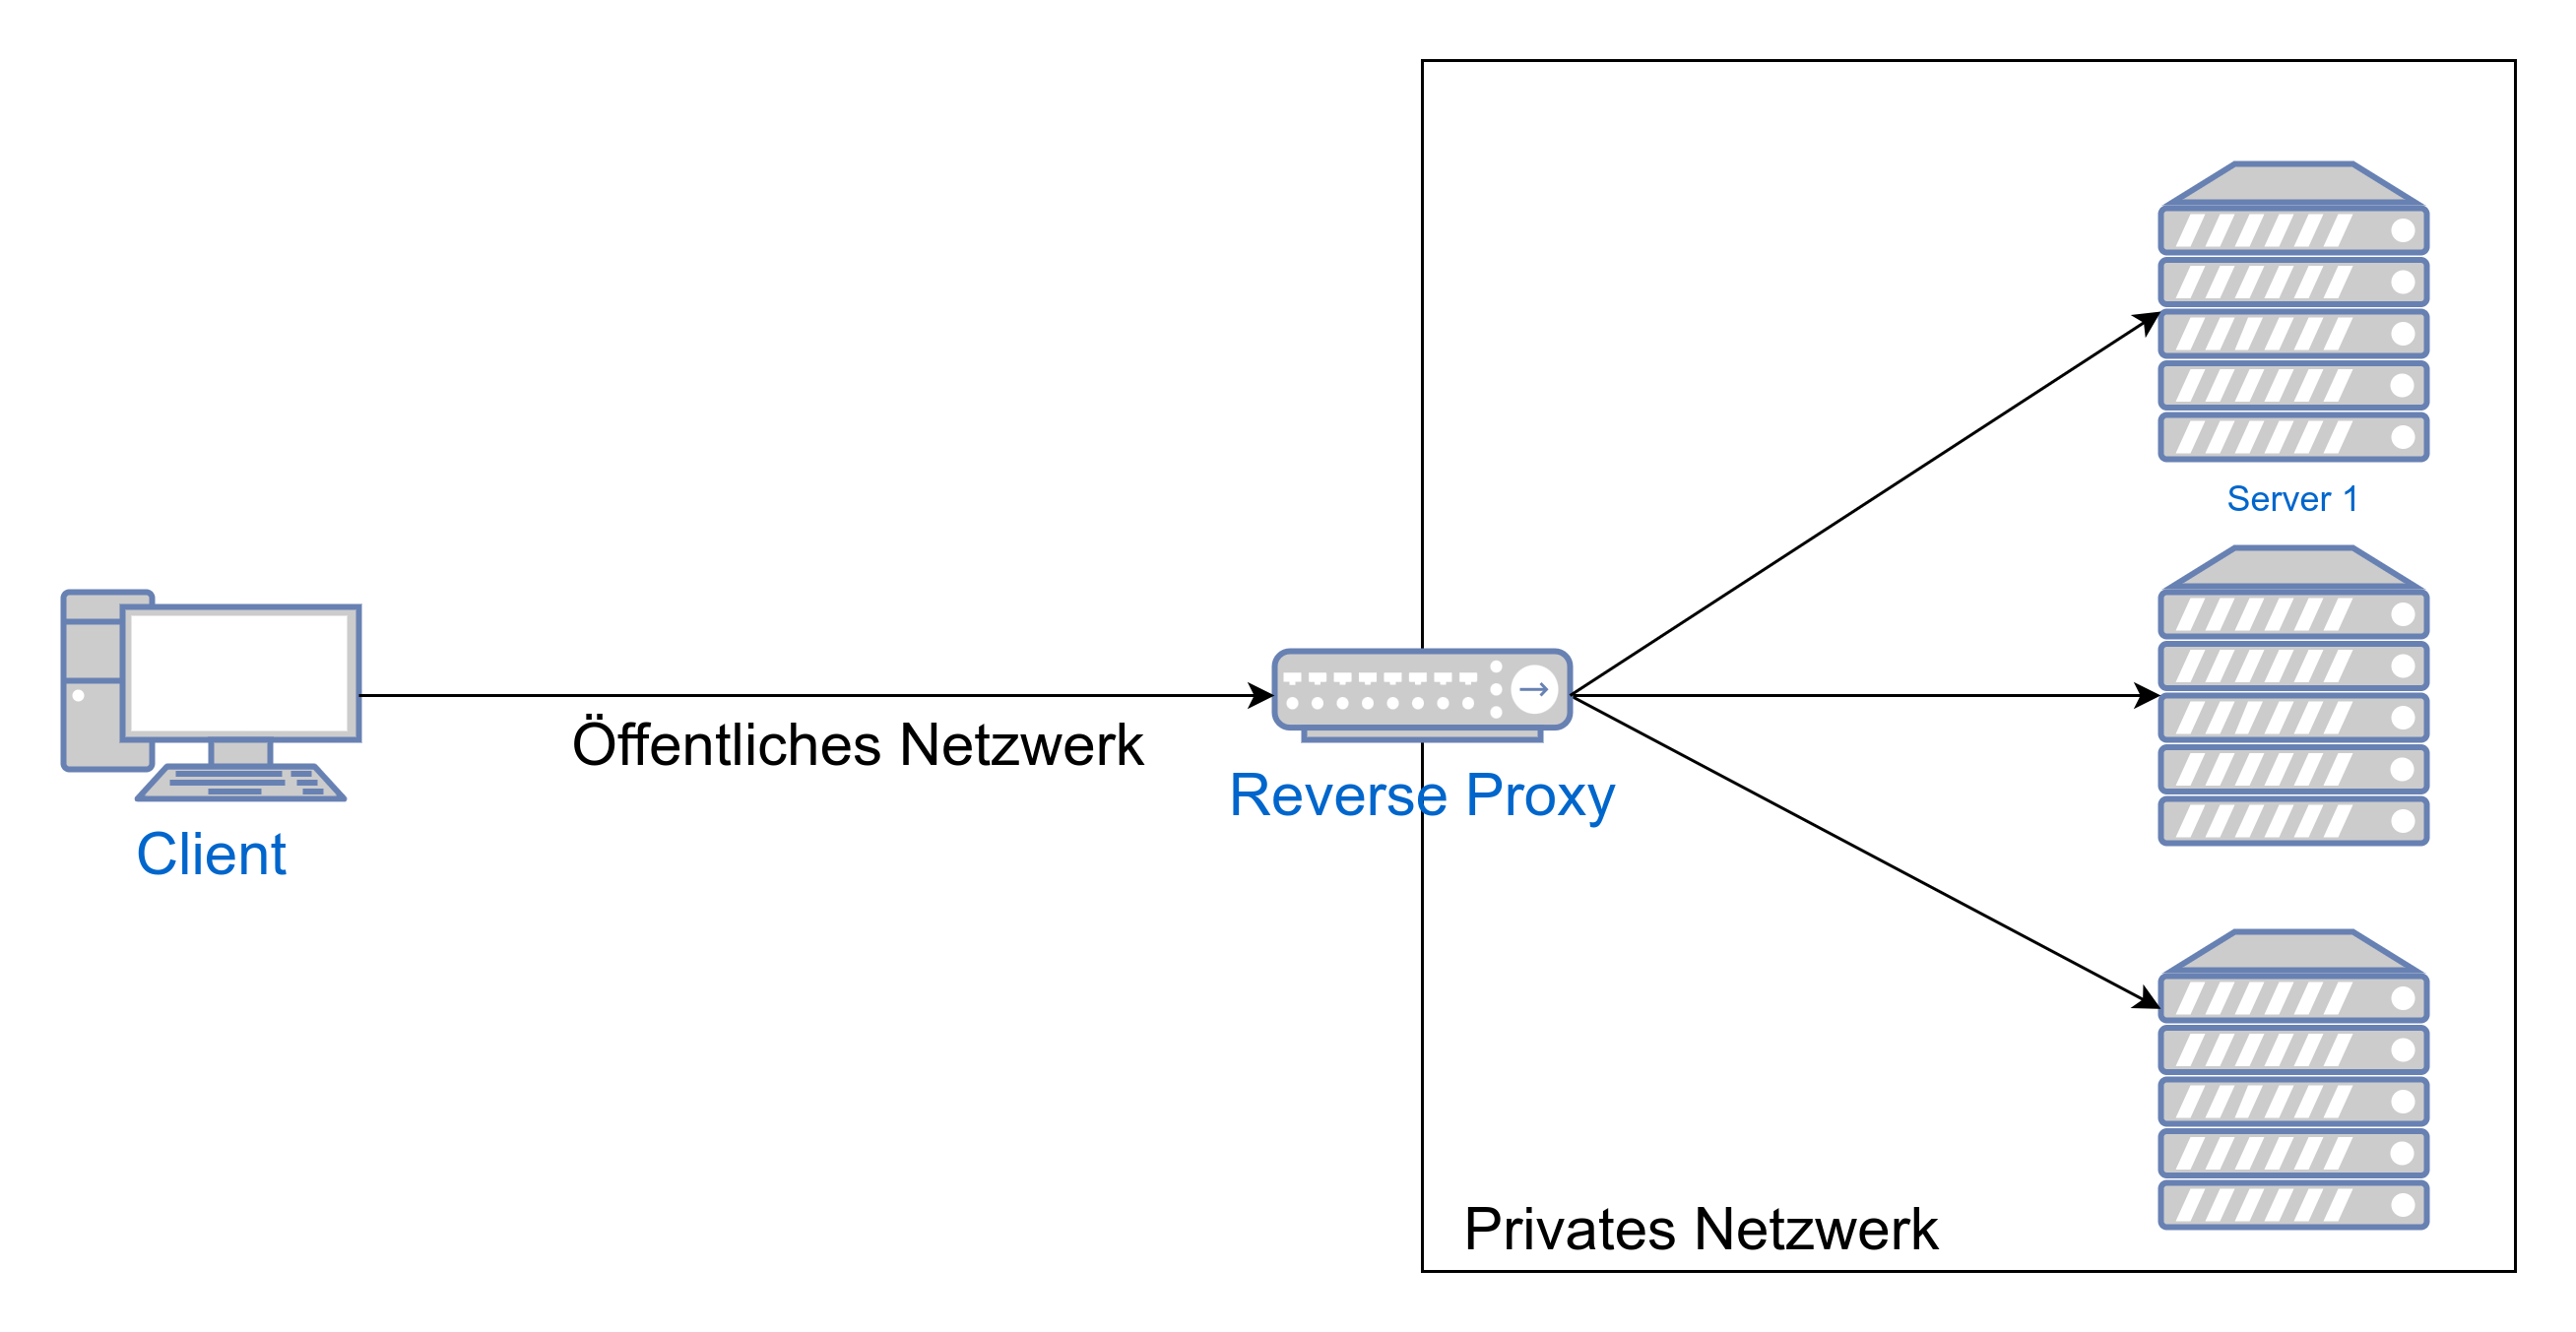
\includegraphics[width=0.9\textwidth]{./images/reverse-Proxy.png}
    \caption{Schematische Darstellung eines Reverse Proxies}
    \floatfoot{Quelle: Eigene Darstellung}
    \label{fig:revprox}
\end{figure}

Hieraus ergeben sich einige positive Sicherheitsaspekte.
Da einem Reverse Proxy Kommunikation unverschlüsselt vorliegt kann diese Inspiziert werden.
Anwendungen die Netzwerksicherheit auf Layer 4 betreiben operieren als Reverse Proxy um tief in Netzwerkverkehr blicken zu können.
Eine \ac{waf} kann konzeptionell als Modul auf einem Reverse Proxy betrachtet werden\cite{WasIstReverse}.

\pagebreak